\documentclass[varwidth]{standalone}
\usepackage{tikz}
\usetikzlibrary{datavisualization}
\usetikzlibrary{datavisualization.formats.functions}

\usepackage{pgfplots}
\usepackage{pgfplotstable}
\pgfplotsset{compat=newest}
\colorlet{negro}{black}
\colorlet{gris}{black!70}
\colorlet{rojo}{red!70!black}
\colorlet{rojol}{red}

\begin{document}
	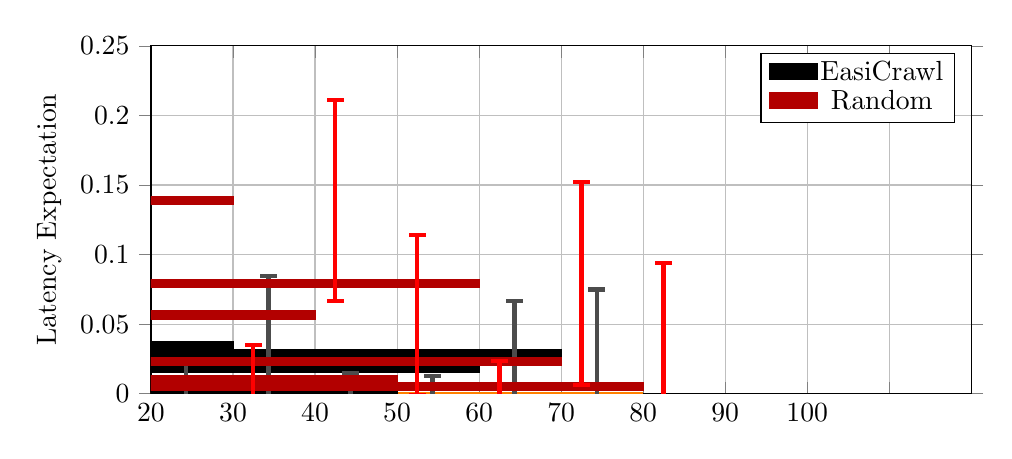
\begin{tikzpicture}
	\begin{axis}[%xscale = 1.45,
	width=12cm, height=6cm,
	scaled ticks=false, tick label style={/pgf/number format/fixed},
	xbar, 
	xmin = 1, xmax = 11,
	ymin = 0, ymax = 0.25,
	ytick = {-0.10, -0.05, 0.00, 0.05, 0.10, 0.15, 0.20, 0.25},
	ylabel = Latency Expectation,	
	xticklabels = {10,20,...,100},
	%ybar interval=0.5,
	bar width=3pt,
	grid = major,
	legend style={cells={anchor=center, fill}, nodes={inner sep=1, below=-1.1ex}}, area legend
	]
	\draw [orange, very thick] (axis cs:0,0) -- (axis cs:7,0);
	\addplot[color = negro, fill = negro, 
	error bars/.cd,
	y dir=both,
	y explicit,
	error bar style={line width=1.5pt, gris, xshift=4.5mm},
	error mark options = {
		rotate = 90, 
		line width=1.5pt, 
		mark size = 3pt, 
		gris,
	}
	]
	coordinates{(1,-0.011097) +- (0,0.0380683)
		(2,0.0393206) +- (0,0.050079)
		(3,-0.019293) +- (0,0.0389844)
		(4,0.0078975) +- (0,0.0097073)
		(5,0.0234860) +- (0,0.0481639)
		(6,0.0336061) +- (0,0.0462397)
		(7,0)};
	\addplot [color = rojo, fill = rojo,
	error bars/.cd,
	y dir=both,
	y explicit,
	error bar style={line width=1.5pt, rojol, xshift=13mm},
	error mark options = {
		rotate = 90, 
		line width=1.5pt, 
		mark size = 3pt, 
		rojol}
	]
	coordinates{(1,-0.025222) +- (0,0.055507)
		(2,0.1337832) +- (0,0.0720284)
		(3,0.0517127) +- (0,0.0574637)
		(4,0.0053732) +- (0,0.0129013)
		(5,0.0741801) +- (0,0.0731692)
		(6,0.0181164) +- (0,0.0709312)
		(7,0)};
	\addlegendentry{EasiCrawl}
	\addlegendentry{Random}
	\end{axis}
	\end{tikzpicture}
\end{document}